% 正文待 P5.3 撰写，表与图由 exp1/scripts/export_tables.py 生成。
\section{实验结果}

\subsection{主结果}

待撰写。

\begin{table}[htbp]
\centering
\caption{五种方法在两个测试集上的准确率与 Wilson 区间}
\label{tab:main}
\begin{tabular}{lSlSl}
\toprule
\multirow{2}{*}{方法} & \multicolumn{2}{c}{GSM8K} & \multicolumn{2}{c}{ARC-Challenge} \\
\cmidrule(lr){2-3}\cmidrule(lr){4-5}
 & {准确率} & {95\% 区间} & {准确率} & {95\% 区间} \\
\midrule
基座 & 0.6020 & 0.5753--0.6281 & 0.5205 & 0.4919--0.5490 \\
全参微调 & 0.5125 & 0.4855--0.5394 & 0.5444 & 0.5158--0.5727 \\
LoRA & 0.4435 & 0.4169--0.4705 & 0.5734 & 0.5449--0.6014 \\
P-Tuning v2 & 0.3829 & 0.3570--0.4094 & 0.4991 & 0.4706--0.5277 \\
自研方法 & 0.5701 & 0.5432--0.5966 & 0.5546 & 0.5260--0.5828 \\
\bottomrule
\end{tabular}
\end{table}


\begin{figure}[htbp]
  \centering
  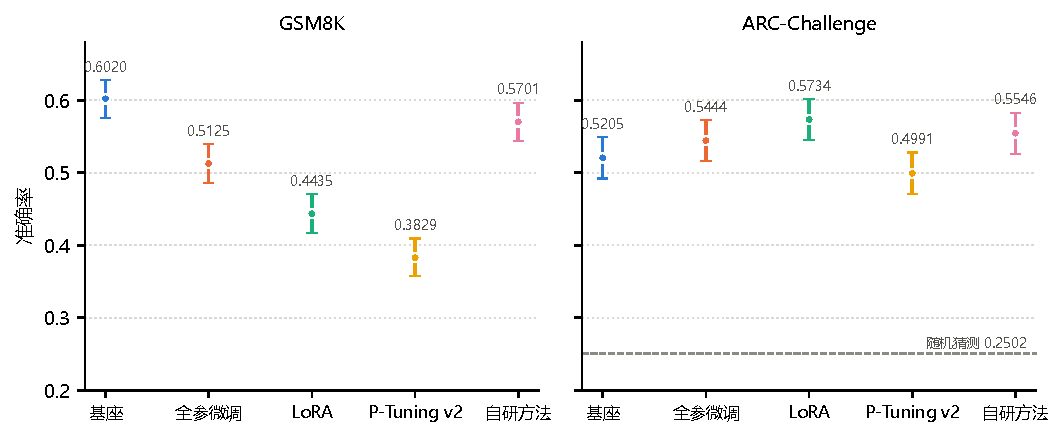
\includegraphics[width=\linewidth]{fig1-accuracy.pdf}
  \caption{五种方法在两个测试集上的准确率与 95\% Wilson 区间}
  \label{fig:accuracy}
\end{figure}

\subsection{配对检验}

待撰写。

\begin{table}[htbp]
\centering
\caption{同批测试样本上的配对检验，差值为前者减后者}
\label{tab:paired}
\begin{tabular}{lSlSl}
\toprule
\multirow{2}{*}{对比} & \multicolumn{2}{c}{GSM8K} & \multicolumn{2}{c}{ARC-Challenge} \\
\cmidrule(lr){2-3}\cmidrule(lr){4-5}
 & {差值} & {Holm $p$} & {差值} & {Holm $p$} \\
\midrule
全参微调\ 相对\ 基座 & -8.95 & $<$0.0001 & 2.39 & 0.3319 \\
LoRA 相对\ 基座 & -15.85 & $<$0.0001 & 5.29 & 0.0012 \\
P-Tuning v2 相对\ 基座 & -21.91 & $<$0.0001 & -2.13 & 0.3319 \\
自研方法\ 相对\ 基座 & -3.18 & 0.0166 & 3.41 & 0.0218 \\
自研方法\ 相对\ LoRA & 12.66 & $<$0.0001 & -1.88 & 0.3357 \\
自研方法\ 相对\ 全参微调 & 5.76 & 0.0003 & 1.02 & 0.5675 \\
自研方法\ 相对\ P-Tuning v2 & 18.73 & $<$0.0001 & 5.55 & 0.0032 \\
\bottomrule
\end{tabular}
\begin{minipage}{\linewidth}
\vspace{0.3em}\footnotesize 差值单位为百分点。$p$ 为 McNemar 精确检验双侧值，
经同一数据集同一家族内的 Holm 校正。
\end{minipage}
\end{table}


\subsection{输出行为}

待撰写。

\begin{table}[htbp]
\centering
\caption{输出行为指标，截断与抽取失败均按样本计}
\label{tab:behavior}
\begin{tabular}{lSSSS}
\toprule
方法 & {GSM8K 均长} & {ARC 均长} & {ARC 截断率} & {ARC 抽取失败率} \\
\midrule
基座 & 208.4 & 12.7 & 0.0009 & 0.0000 \\
全参微调 & 93.5 & 279.7 & 0.4514 & 0.0768 \\
LoRA & 108.7 & 174.4 & 0.2696 & 0.0333 \\
P-Tuning v2 & 110.0 & 26.3 & 0.0034 & 0.0904 \\
自研方法 & 185.9 & 23.6 & 0.0000 & 0.0026 \\
\bottomrule
\end{tabular}
\begin{minipage}{\linewidth}
\vspace{0.3em}\footnotesize 均长单位为 token。抽取失败率取 v3 口径。
\end{minipage}
\end{table}


\begin{figure}[htbp]
  \centering
  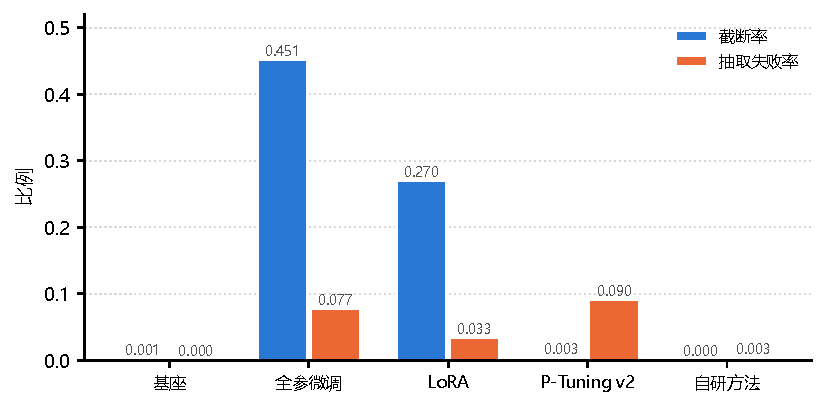
\includegraphics[width=0.92\linewidth]{fig2-behavior.pdf}
  \caption{ARC-Challenge 上五种方法的截断率与抽取失败率}
  \label{fig:behavior}
\end{figure}

\subsection{正则系数扫描}

待撰写。

\begin{table}[htbp]
\centering
\caption{正则系数五档扫描在 400 条开发集上的读数}
\label{tab:beta}
\begin{tabular}{SSSS}
\toprule
{系数} & {正确数} & {准确率} & {生成均长} \\
\midrule
0.05 & 196 & 0.4900 & 106.0 \\
0.2 & 195 & 0.4875 & 110.1 \\
0.8 & 243 & 0.6075 & 153.3 \\
1.6 & 241 & 0.6025 & 180.7 \\
3.2 & 233 & 0.5825 & 191.7 \\
\bottomrule
\end{tabular}
\begin{minipage}{\linewidth}
\vspace{0.3em}\footnotesize 正确数以 400 条为分母，均长单位为 token。
\end{minipage}
\end{table}


\begin{figure}[htbp]
  \centering
  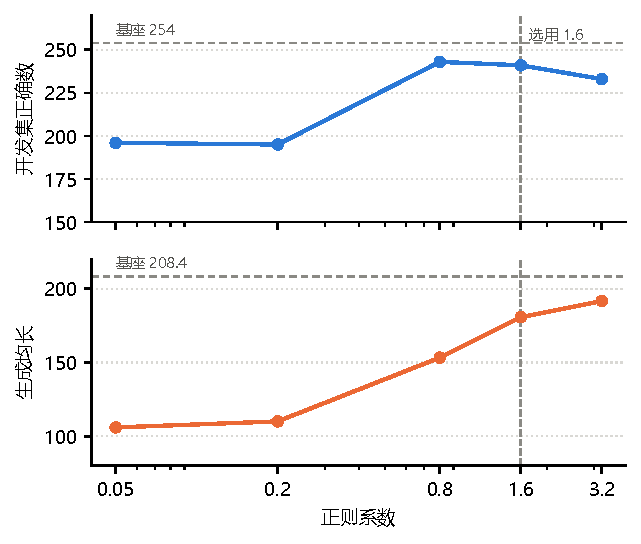
\includegraphics[width=0.78\linewidth]{fig3-beta.pdf}
  \caption{正则系数五档扫描的开发集正确数与生成均长}
  \label{fig:beta}
\end{figure}

\subsection{通用文本困惑度}

待撰写。

\begin{table}[htbp]
\centering
\caption{五个模型在 WikiText-2 前二百万 token 上的困惑度}
\label{tab:ppl}
\begin{tabular}{lSS}
\toprule
方法 & {困惑度} & {相对基座} \\
\midrule
基座 & 24.34 & 1.000 \\
全参微调 & 27.67 & 1.137 \\
LoRA & 22.27 & 0.915 \\
P-Tuning v2 & 229.43 & 9.426 \\
自研方法 & 23.18 & 0.952 \\
\bottomrule
\end{tabular}
\begin{minipage}{\linewidth}
\vspace{0.3em}\footnotesize P-Tuning v2 的前缀仅在对话模板格式的输入上训练，
与无模板语料不匹配，其读数只作描述，不参与方法排序。
\end{minipage}
\end{table}


\subsection{抽取口径的稳健性}

待撰写。
